\documentclass[10pt]{article}
\usepackage[margin=0.85in]{geometry}
\usepackage{amsmath,booktabs,graphicx,hyperref,xcolor,enumitem}
\hypersetup{colorlinks=true,linkcolor=blue,urlcolor=blue,citecolor=blue}
\setlength{\parskip}{0.4em}
\setlength{\parindent}{0pt}
\setlist{nosep}
\newcommand{\WeatherRatio}{0.9995}
\newcommand{\WeatherComparison}{meets}
\newcommand{\InferenceBound}{0.897}
\newcommand{\TrainingBound}{0.815}
\newcommand{\InferenceControlRatio}{1.84}
\newcommand{\TrainingControlRatio}{0.90}
\newcommand{\SpeedGate}{passes}
\newcommand{\ConstantRatio}{0.99241}
\newcommand{\ZonalRatio}{0.93466}
\newcommand{\ConstantAmplitude}{0.00380}
\newcommand{\WarmTracerRatio}{0.00232}
\newcommand{\WarmTracerPeak}{0.989}
\newcommand{\WarmTracerMass}{+8.61}
\newcommand{\DataUpstream}{391.4}
\newcommand{\DataOptimized}{260.1}
\newcommand{\DataSpeedup}{1.50}

\title{PARADIS with spherical DISCO convolutions\\\large Native PyTorch port and compact CPU reproduction}
\author{Reproduction workspace: \texttt{yikwill/paradis-spherical}}
\date{October 2026}
\begin{document}
\maketitle
\begin{abstract}
This work ports the public PARADIS implementation to native PyTorch, replaces all
spatial convolutions with selectable DISCO operators, removes learned spatial bias
maps, and restricts explicit coordinate inputs to unnormalized sine of latitude.
The unchanged upstream trainer and the native orchestration agree exactly on a
small deterministic output/loss/gradient/AdamW fixture. Additional checks cover
spherical operators, temporal splits, autoregression, checkpoint continuation,
distributed CPU execution, and real-data forecast writing. Experiments use a full
$721\times1440$ tracer grid and a compact, paired 2,000-update weather comparison
on real ERA5. These bounded CPU experiments do not reproduce the paper's full
weather training or establish GPU performance. All measured outcomes, including
unsuccessful tracer fits and performance gates, are retained.
\end{abstract}

\section{Scope and source}
The reference is Pereira et al.'s \emph{Learning to Advect}, version 1, whose
Figure 3 compares a depth-three U-Net to a 20-parameter neural semi-Lagrangian
(NSL) operator \cite{paradis}. As requested for this fork, the replacement panel
uses the complete compact PARADIS architecture, including its encoders, two
advection--diffusion--reaction blocks, gates, and decoder. It is therefore a
modified experiment, not an exact reconstruction of the paper's small NSL model.

The complete upstream repository and history are retained at commit
\texttt{9a6f4b7d0dadfb80918ff8929bd92b6a5da2bcc5}. The unchanged reference is a detached
worktree. The primary implementation commit is \texttt{58f5fbf}; later commits
contain additional checks, experiment drivers, measurements, and this report.
Saved weather configurations and provenance files identify the training source.
The private repository is \url{https://github.com/yikwill/paradis-spherical}.

The accepted budget is 12 CPU experiment wall-hours, excluding installation,
data download, and report compilation. Four GPU-hours remain reserved because
supported GPU hardware was unavailable. The execution ledger in
\texttt{results/budget.json} records the actual experiment interval and individual
run durations. Concurrent run durations must not be summed as elapsed wall time.

\section{Implementation and numerical verification}
\subsection{Native orchestration}
The native trainer retains the upstream autoregressive feature layout, loss scale,
truncated backpropagation, fixed accumulation denominator, AdamW parameter groups
(including the gate learning-rate multiplier), and warmup--steady--decay schedule.
It implements validation, clipping, early stopping, atomic checkpoints, and
\texttt{torchrun} distribution without Lightning or TensorBoard. Checkpoints save
optimizer/scheduler state, random generators, progress, grid, feature order, and
normalization metadata. Exact continuation rejects incompatible training settings
or distributed world size. Forecast horizons can change without changing weights.

Static encodings are reused within a truncation chunk and across a forecast through
an explicit argument. This avoids caching activations across unrelated batches.
The data cache holds raw arrays; every sample is copied before normalization.
Preloaded sample access bypasses xarray/Dask indexing and reuses time/solar forcings.
A configured memory budget bounds preload allocation.

\begin{table}[ht]
\centering\small
\begin{tabular}{lp{9.1cm}}
\toprule
Check & Verified result \\
\midrule
Unchanged upstream port & Two autoregressive steps, two accumulated batches: maximum output, loss, gradient, and AdamW-update error all zero. \\
DISCO CPU contraction & Matches the library operator and first gradients; float64 reference error about $10^{-15}$; finite-difference input gradient passes. \\
Spherical geometry & Longitude-roll equivariance, scalar pole rows, and total quadrature weight $4\pi$. \\
Architecture & All nine spatial convolutions in the two-block compact model replaced; only $1\times1$ Conv2d layers remain in DISCO mode; no learned spatial bias factors. \\
Static-feature reuse & Losses and parameter gradients match recomputation for truncation lengths 1, 2, and 3. \\
Checkpoint continuation & Bitwise agreement for both backends; actual fit-loop interruption/resume crosses an epoch boundary. \\
Data and loss & Complete-window split isolation, one/two-frame order, normalization and cache immutability; all 97 named loss weights. \\
Native execution & Two CPU ranks with accumulation, validation and checkpointing; real ERA5 forecast to incremental Zarr, including horizon changes and lead-time coordinates. \\
Compilation & Full weather-shaped output and gradient checks pass before enabling compilation; output error below $5\times10^{-7}$. \\
\bottomrule
\end{tabular}
\caption{Runnable checks are in \texttt{tests/}; compilation checks are in \texttt{experiments/tune\_compile.py}. These are scoped checks, not evidence of untested GPU behavior.}
\end{table}

Two upstream correctness changes are intentional and separate from the exact port
fixture. First, the original loader could include targets beyond a training split's
end date. Complete input/target windows are now contained in each split. Second,
common-first channel reordering interleaves surface variables before some atmospheric
outputs, so pressure weighting by position was incorrect. Weights now use feature
names and pressure suffixes. For example, a surface wind received weight 0.2 instead
of 1, while a 925-hPa vertical-velocity output received 0.1 instead of 0.0925. The
upstream loss formula otherwise remains unchanged. A one-input shape bug and
forecast output-frequency lead times are also corrected; existing forecast stores
are protected from overwrite.

\subsection{DISCO and CPU implementation}
The adapter uses NVIDIA torch-harmonics at
\texttt{6e7648d4435109c8a4ae747a9cd279b6ae3a30ba} \cite{harmonics,disco}.
For an odd spatial width $k$, its piecewise-linear basis shape is $(k,2k+2)$,
yielding $k^2$ learned basis coefficients. The angular support radius is
$k\Delta\phi/2$. Grids include both latitude poles, use an even periodic longitude
count, and preserve these conditions through coarsening. The adapter reverses the
south-to-north data convention for the library and averages scalar pole values.
These checks establish the implemented longitude symmetry; they do not establish
full rotation equivariance of the weather model.

Profiling identified basis-expanded depthwise activations and copies as a CPU
bottleneck. A small C++ operator directly contracts the same quadrature stencil,
without changing the learned basis or geometric weights. Its backward assigns each
channel to one worker, avoiding atomic gradient accumulation. The path is used only
for CPU float32/float64 depthwise layers. Other cases use torch-harmonics. Build
flags enable OpenMP, vectorization, and the current CPU architecture. Higher-order
derivatives are outside the implemented extension interface.

The retained kernel microbenchmarks show roughly $3.3\times$ and $2\times$ training
speedups over the library implementation for the tested large and small layer
shapes. These isolated operator gains are not end-to-end model speedups. Library
fusion and channels-last layout were evaluated and did not consistently improve both
shapes, so they remain disabled. Compilation was retained for the paired weather
runs after numerical checks. Its initial cost was 164--265 seconds in the pilot and
is reported separately from warmed latency.

\section{Tracer reconstruction}
The grid contains 721 latitudes and 1,440 longitudes. The initial tracer is an
isotropic geodesic Gaussian with amplitude 1 and standard deviation $5^\circ$,
centered at $(0^\circ,0^\circ)$. Its analytic target follows a $68^\circ$ great-circle
displacement with initial northeast bearing $45^\circ$. These initialization
settings are explicit fallback assumptions where original experiment details were
unavailable. The objective uses exact latitude-cell areas, including half-cells
at the poles:
\[
 \mathcal{L}=\frac{\sum_{ij} A_i(\hat q_{ij}-q_{ij})^2}{\sum_{ij} A_i}.
\]
The reported relative MSE divides this by the zero-predictor MSE, preventing a
small absolute loss on a mostly empty globe from being mistaken for successful
transport. Signed mass error and prediction extrema are also in the raw results.
The optimal spatially constant prediction has amplitude \ConstantAmplitude\ and
relative MSE \ConstantRatio. Reaching this baseline, even with accurate total
mass, does not demonstrate localization or transport of the Gaussian.

The compact full PARADIS has 8 latent, 4 transported, and 8 static channels, two
processor blocks, and spatial coarsening by 2. A depth-three U-Net with top width 4
is reconstructed from the paper's Figure 19: an entry convolution followed by a
normalized two-convolution residual block at each level. The chosen $3\times3$
kernels, upstream ChannelNorm, unit residual scale, average pooling, and bilinear
upsampling remain implementation assumptions. This version has 46,481 parameters,
versus the paper's stated 45,909; the original toy-experiment code was not recovered.
Earlier plain double-convolution U-Net runs (30,601 parameters) are retained as
auxiliary diagnostics and excluded from the main figure. Both models use seed 42, AdamW with learning rate 0.002,
zero weight decay, and gradient clipping at 1.

The main protocol trains directly against the fixed $68^\circ$ target for up to
500 updates. Separately labelled diagnostics (i) ramp the target over 300 updates
then hold it fixed, and (ii) first train identity transport for 300 updates, ramp
over 600 updates, then hold the target fixed. These are optimization diagnostics,
not substitutions for the main fixed-target result. Time caps and completed update
counts are preserved in each JSON record.

\begin{figure}[p]
\centering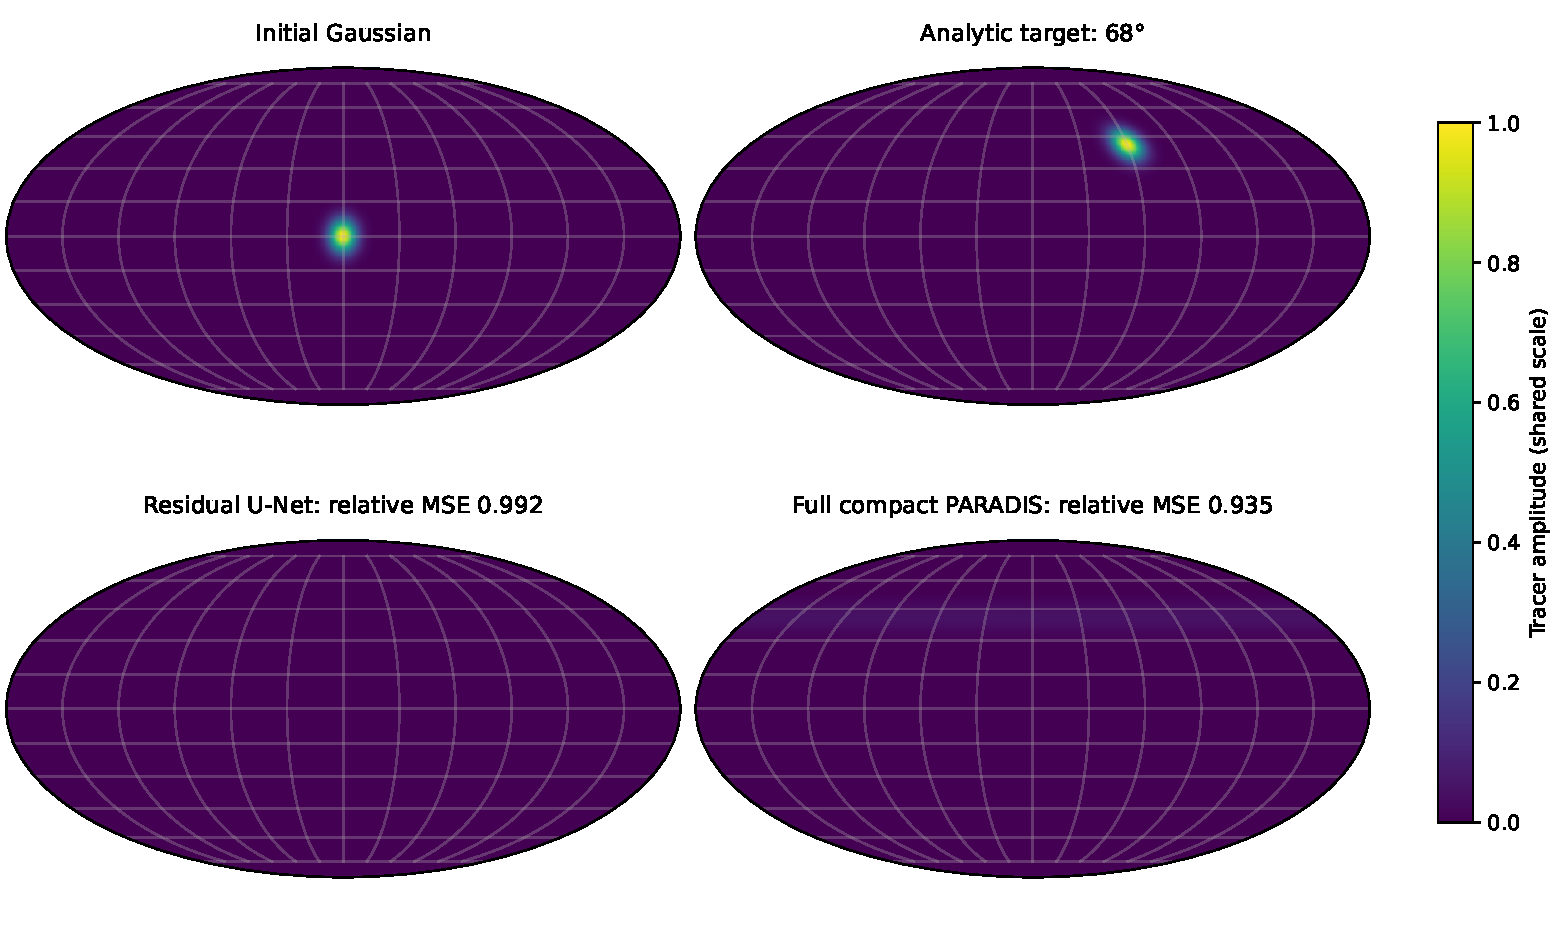
\includegraphics[width=\linewidth]{figures/tracer.pdf}
\caption{Figure 3-style reconstruction under the fixed-target protocol. All maps
use the same amplitude scale and the full grid; the lower-right panel is the
requested compact full PARADIS with DISCO. A relative MSE near 1 indicates little
improvement over predicting zero. Negative/above-one predictions are outside the
shared display range and are quantified in the raw metrics.}
\end{figure}
\begin{table}[ht]
\centering\small
\begin{tabular}{lrrrrrr}
\toprule
Model/protocol & Parameters & Updates & Angle & MSE & Relative MSE & Minutes \\
\midrule
PARADIS + warmup & 3,562 & 1000 & 68.0 & 4.41e-06 & 0.002 & 147.7 \\
PARADIS + ramp & 3,562 & 204 & 46.2 & 0.00207 & 1.091 & 90.3 \\
PARADIS & 3,562 & 500 & 68.0 & 0.00178 & 0.935 & 77.8 \\
U-Net(P) + warmup & 30,601 & 1000 & 68.0 & 0.00189 & 0.992 & 58.7 \\
U-Net(P) + ramp & 30,601 & 400 & 68.0 & 0.00189 & 0.992 & 20.9 \\
U-Net(R) + warmup & 46,481 & 1000 & 68.0 & 0.00189 & 0.992 & 145.9 \\
U-Net(R) + ramp & 46,481 & 400 & 68.0 & 0.00189 & 0.992 & 52.6 \\
U-Net(R) & 46,481 & 500 & 68.0 & 0.00189 & 0.992 & 65.3 \\
U-Net(P) & 30,601 & 500 & 68.0 & 0.00189 & 0.992 & 26.4 \\

\bottomrule
\end{tabular}
\caption{Every attempted tracer protocol is retained. U-Net(R) is the residual
reconstruction and U-Net(P) is the earlier plain diagnostic. ``Ramp'' denotes angular
continuation; ``warmup'' adds identity training. Elapsed optimization time includes
final evaluation, but excludes model/stencil construction. Angle is the last
training target in degrees; a time-capped run may not reach $68^\circ$.}
\end{table}
\begin{figure}[ht]
\centering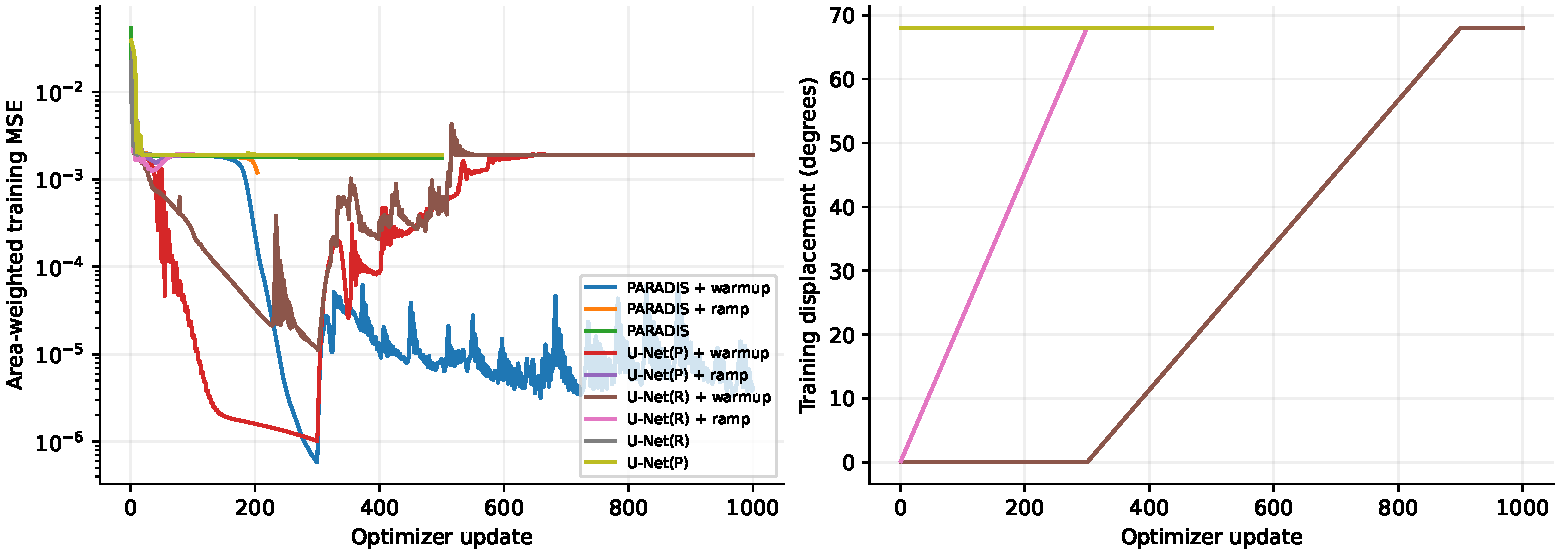
\includegraphics[width=\linewidth]{figures/tracer-learning.pdf}
\caption{Tracer optimization histories and the actual target angle at each update.
Losses during continuation refer to the moving training target; final table errors
always use the $68^\circ$ target.}
\end{figure}

\section{Partial weather comparison}
Real ERA5 data comes from the WeatherBench 2 $121\times240$ equiangular-with-poles
store \cite{wb2}. Training uses all of 2016 (1,464 six-hourly times), and validation
uses January 2017 (124 times). Two input frames and one forecast step yield 1,462
training and 122 validation windows. The full configured pressure-level/variable
selection gives 97 output channels. Cartesian wind conversion follows upstream;
physical constants and fractional land--sea mask are retained. Lossless storage
and training-only normalization statistics avoid an additional quantization change.
The source URI, coordinate checks, and preparation provenance are in
\texttt{results/data-manifest.json}.

Both optimized models have 111,638 parameters, two processor blocks, 64 latent,
32 transported, and 32 static channels. Training is paired by seed, sample order,
update count, AdamW hyperparameters, and learning-rate schedule. The initial
learning rate is $5\times10^{-4}$, Adam betas are $(0.9,0.95)$, and weight decay is
0.01. Twenty warmup updates precede the steady phase; the last 20\% decay linearly.
Every 200 updates, all 122 validation windows are evaluated using the configured
latitude-, pressure-, and variable-weighted reversed-Huber loss. The common count
of 2,000 updates was fixed before comparative training.

\begin{table}[ht]
\centering
\begin{tabular}{lrrrr}
\toprule
Backend & Updates & Final validation & Best validation & Fit minutes \\
\midrule
conv2d & 2,000 & 0.11408 & 0.11408 & 61.0 \\
disco & 2,000 & 0.11402 & 0.11402 & 90.4 \\

\bottomrule
\end{tabular}
\caption{Paired short weather runs. Fit time includes compilation, training,
validation, and checkpoint writes, and excludes dataset preload/model construction.}
\end{table}
The final DISCO/Conv2d validation-loss ratio is \WeatherRatio. The predeclared
\emph{descriptive} comparability threshold is 1.10. This is one short, single-seed
comparison, approximately 1.37 passes over the training windows; it is not a
statistical equivalence test or evidence of full-scale forecasting skill. The
short run, changed architecture, resolution, coordinate inputs, and corrected
loss weighting prevent direct comparison with the paper's published scores.

\begin{table}[ht]
\centering
\begin{tabular}{lrr}
\toprule
Predictor & $z_{500}$ RMSE ($\mathrm{m^2\,s^{-2}}$) & $T_{2\mathrm{m}}$ RMSE (K) \\
\midrule
persistence & 236.52 & 2.536 \\
conv2d & 167.87 & 3.174 \\
disco & 170.14 & 3.129 \\

\bottomrule
\end{tabular}
\caption{Six-hour RMSE of final checkpoints, pooled across all 122 January
validation windows with cosine-latitude weighting. Persistence carries the last
input field forward. These physical-unit scores contextualize the aggregate loss;
they are not the paper's long-lead forecast evaluation.}
\end{table}

\begin{figure}[ht]
\centering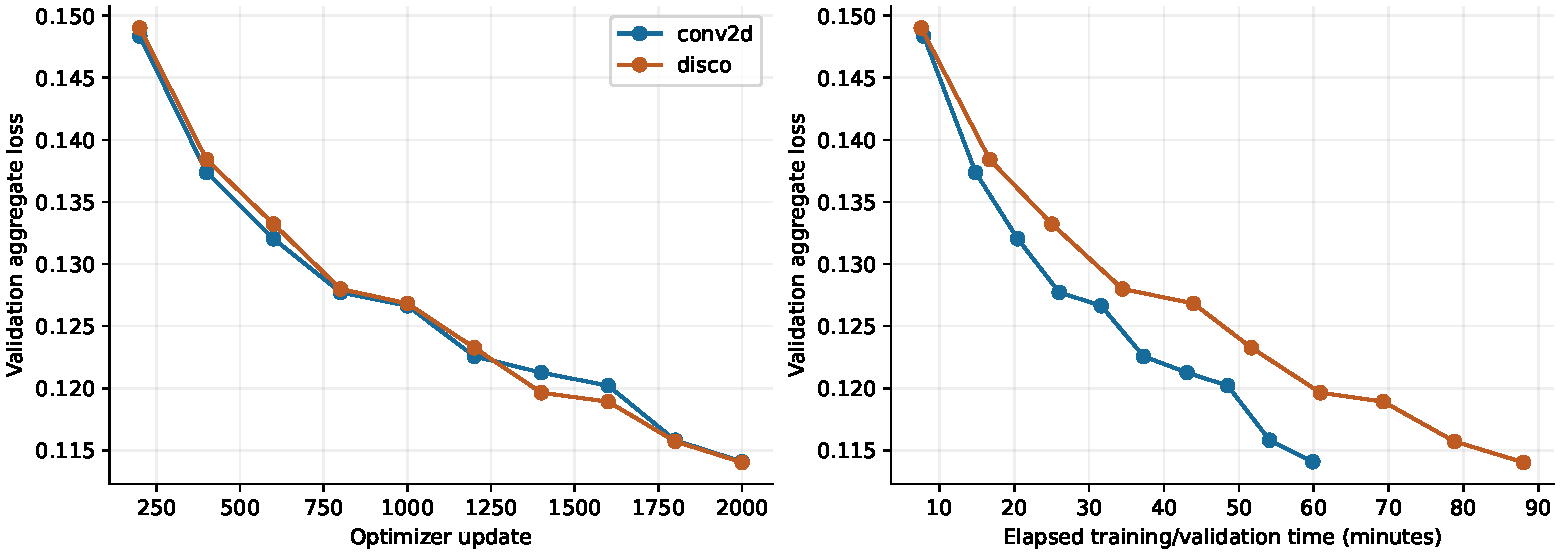
\includegraphics[width=\linewidth]{figures/weather-learning.pdf}
\caption{Validation loss versus equal update count and elapsed time. Logged time
is sampled immediately before each validation pass, so each point excludes that
pass's duration; the table uses total fit wall time.}
\end{figure}

\section{Performance measurements and limits}
The host is a dual-socket Intel Xeon Gold 5220R (48 physical cores, 96 logical CPUs),
with approximately 754 GiB RAM. The CPU environment uses Python 3.11.17 and
PyTorch 2.14.1+cpu. The final latency experiment uses four pinned CPU threads,
with our other training jobs finished. External host load and operating-system
noise remain uncontrolled.

The benchmark compares the pinned upstream model, optimized Conv2d, and optimized
DISCO using identical full-feature synthetic inputs, grid $121\times240$, batch
size 1, two blocks, 64 latent/32 transported channels, and matched static widths
128/64. The upstream model retains its spatial bias maps. The input width is
held fixed to isolate execution; this is not the complete original coordinate
configuration. Training includes forward, loss, backward, and AdamW in the same
native harness, not the Lightning framework. The optimized variants are compiled;
upstream is eager. Two warmup calls per workload/variant and construction/compile
time are reported outside the steady-state measurements.

Each measurement block randomizes variant order. Twenty blocks are retained.
Bootstrap resampling of paired blocks (10,000 draws) estimates a one-sided 95\%
upper bound on the ratio of median latencies. The strict no-slowdown criterion is
an upper bound at most 1 for \emph{both} inference and training. It is a gate for
this CPU workload, not a universal performance guarantee.

\begin{table}[ht]
\centering
\begin{tabular}{llrr}
\toprule
Workload & Variant & Median seconds & DISCO/upstream upper 95\% \\
\midrule
inference & upstream & 1.9688 & --- \\
inference & conv2d & 0.5495 & --- \\
inference & disco & 1.0132 & 0.897 \\
training & upstream & 3.6989 & --- \\
training & conv2d & 2.7503 & --- \\
training & disco & 2.4721 & 0.815 \\

\bottomrule
\end{tabular}
\caption{Warmed, interleaved final measurements. Bounds are shown only on the
DISCO rows. Raw samples and both upstream/control comparisons are committed.}
\end{table}
The inference upper bound is \InferenceBound; the training upper bound is
\TrainingBound. The JSON \texttt{no\_slowdown} fields give the gate outcomes.
A failed bound is retained as a failed target, even when the point estimate or an
isolated kernel is faster. No CPU result establishes GPU parity.

\begin{figure}[ht]
\centering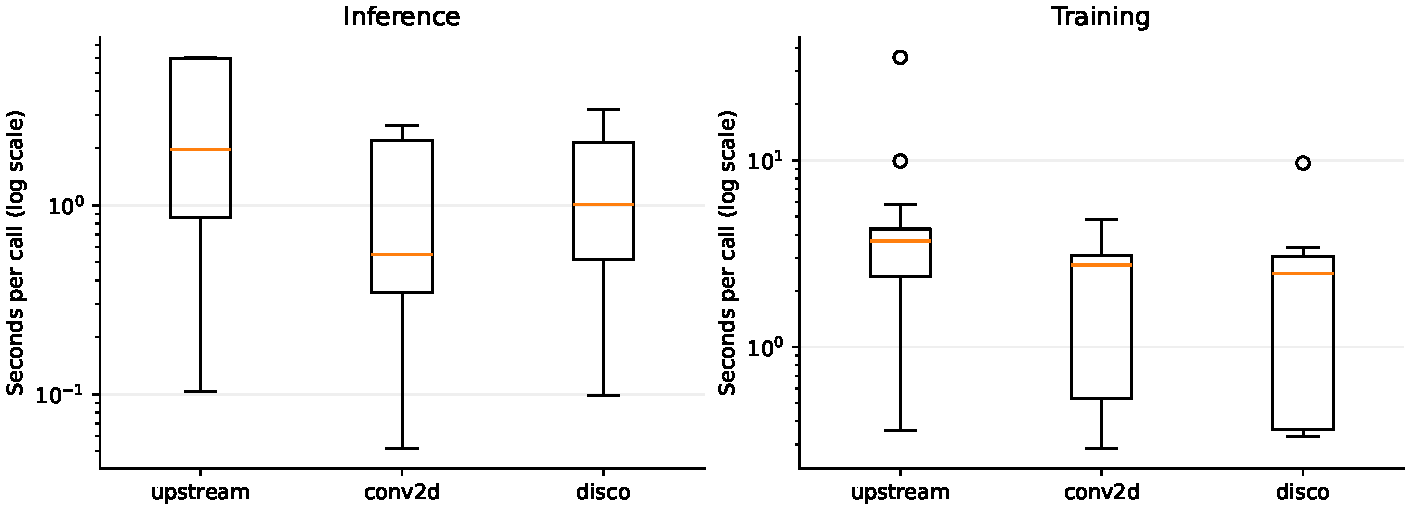
\includegraphics[width=.9\linewidth]{figures/latency.pdf}
\caption{Final latency sample distributions. Compilation and setup are excluded
from these boxes and retained separately in the raw result file.}
\end{figure}

Fresh-process memory measurements in \texttt{results/memory-*.json} report resident
peaks including Python, libraries, model construction, and compilation. They are
not isolated tensor-allocation peaks.
\begin{table}[ht]
\centering
\begin{tabular}{lrr}
\toprule
Variant & Import peak (GiB) & Full process peak (GiB) \\
\midrule
upstream & 0.36 & 1.16 \\
conv2d & 0.36 & 1.02 \\
disco & 0.36 & 1.04 \\

\bottomrule
\end{tabular}
\caption{Separate processes, three training updates each, four CPU threads;
optimized variants compiled, upstream eager.}
\end{table}

The separate data-loading benchmark compares
preloaded January samples at matching initialization times and checks numerical
agreement of dynamic fields and forcings. Constant coordinate channels differ
intentionally. Setup timings include reads with an uncontrolled filesystem cache.
Median sample time is \DataUpstream\ ms upstream and \DataOptimized\ ms optimized,
a measured speedup of \DataSpeedup$\times$; dynamic/forcing values agree exactly.
Pilot profiles and tuning trials are retained for audit; the earliest pilot used
only five output features and must not be compared directly to the final
97-output-channel latency measurements.

\section{Reproduction and remaining limitations}
The README provides commands for environment construction, data preparation,
training, forecast writing, each regression check, benchmarks, and tracer runs.
Rebuild figures and PDF with:
\begin{verbatim}
python report/make_figures.py
cd report
latexmk -pdf -interaction=nonstopmode -halt-on-error report.tex
\end{verbatim}
The existing locked environment was exercised, but a second clean installation
was not used as a verification step. Dataset stores and model checkpoints remain
local and are excluded from Git; configurations, histories, numerical summaries,
figures, source, and the PDF are committed. The full-resolution tracer field files
are available in the local data directory and generated by the experiment driver.

This work verifies a native CPU implementation and a bounded modified experiment.
The full upstream training scale, original toy-model code, multiple training seeds,
long-range weather skill, and all CUDA paths remain unverified. These limitations
must accompany any reuse of the reproduction's numerical comparisons.

\begin{thebibliography}{9}
\bibitem{paradis} Pereira et al. \emph{Learning to Advect: A Neural Semi-Lagrangian
Architecture for Weather Forecasting}. arXiv:2601.21151v1.
\url{https://arxiv.org/html/2601.21151v1}.
\bibitem{harmonics} NVIDIA. \emph{torch-harmonics}, pinned source revision listed above.
\url{https://github.com/NVIDIA/torch-harmonics}.
\bibitem{disco} Ocampo, Price, and McEwen. \emph{Scalable and Equivariant Spherical
CNNs by Discrete-Continuous (DISCO) Convolutions}. arXiv:2209.13603.
\url{https://arxiv.org/abs/2209.13603}.
\bibitem{wb2} Google Research. \emph{WeatherBench 2 datasets}.
\url{https://weatherbench2.readthedocs.io/en/latest/data-guide.html}.
\end{thebibliography}
\end{document}
